\documentclass[conference]{IEEEtran}
\bibliographystyle{IEEEtran}
\usepackage[margin=0.75in, top=1in, bottom=1in]{geometry}
\usepackage{cite}
\usepackage{amsmath,amssymb,amsfonts}
\usepackage{graphicx}
\usepackage{textcomp}
\usepackage{xcolor}
\usepackage{booktabs}
\usepackage{multirow}
\usepackage{array}
\usepackage{url}
\usepackage{titlesec}
\usepackage{abstract}
\usepackage{tikz}
\usetikzlibrary{arrows.meta, positioning, shapes.geometric, fit, backgrounds, calc}
\usepackage{hyperref}
\hypersetup{colorlinks=true, linkcolor=blue, citecolor=blue, urlcolor=blue}

% IEEE-style section formatting
\titleformat{\section}{\normalfont\bfseries\scshape\centering}{\Roman{section}.}{0.5em}{}
\titleformat{\subsection}{\normalfont\itshape}{\Alph{subsection}.}{0.5em}{}
\titleformat{\subsubsection}{\normalfont\itshape}{}{0em}{}
\titlespacing{\section}{0pt}{8pt}{4pt}
\titlespacing{\subsection}{0pt}{6pt}{2pt}

% Compact abstract
\renewcommand{\abstractnamefont}{\normalfont\bfseries}
\setlength{\absleftindent}{0pt}
\setlength{\absrightindent}{0pt}

% Shared TikZ styles
\tikzset{
  block/.style={rectangle, rounded corners=2pt, draw=black!70,
                fill=#1, text=white, font=\scriptsize\bfseries,
                minimum width=1.1cm, minimum height=0.52cm,
                inner sep=2.5pt, align=center},
  block/.default=black!60,
  arr/.style={-{Stealth[length=4pt]}, thick, black!70},
  lbl/.style={font=\tiny, black!60},
  grpbox/.style={draw=black!30, dashed, rounded corners=3pt,
                 fill=black!4, inner sep=4pt},
}

\begin{document}
\title{\fontsize{18pt}{22pt}\selectfont
To Synthesize or to Reconstruct? A Comparative Study of GAN-Based Augmentation and Reconstruction-Based Anomaly Detection for Financial Fraud Detection }

\author{
  Kipngeno Koech (bkoech) \quad Bellah Ellam (bellam) \quad Francis Waithaka (fwaithak) \\
  \textit{Carnegie Mellon University}
}

\maketitle

%--------
\begin{abstract}
Credit card fraud detection is a critical machine learning challenge
characterized by extreme class imbalance: fraudulent transactions comprise
only 0.172\% of the Kaggle Credit Card Fraud Dataset (492 of 284,807
transactions). This paper presents a rigorous, unified comparative study of
two deep learning paradigms for addressing this imbalance. Pipeline~A
employs generative data augmentation, training three GAN variants -
R-GAN, T-GAN, and CTGAN - to synthesize minority-class samples for a
downstream LightGBM classifier. Pipeline~B employs reconstruction-based
anomaly detection, training three semi-supervised models - GANomaly,
Skip-GANomaly, and f-AnoGAN - exclusively on normal transactions and
identifying fraud through reconstruction error. All models are evaluated
under identical feature engineering and validation conditions on the same
held-out fraud set. Results across all six completed models show that
Pipeline~A substantially outperforms Pipeline~B on F1: R-GAN + LightGBM
achieves F1~=~0.9954 and AUROC~=~0.9999, while the best reconstruction
model, Skip-GANomaly, achieves F1~=~0.8742 and AUROC~=~0.9821. Within
Pipeline~B, f-AnoGAN achieves the highest AUROC (0.9907) and recall
(0.9390), confirming the inference-speed design objective at production
throughput. Statistical significance of cross-paradigm F1 differences
is assessed via the Wilcoxon Signed-Rank Test.
\end{abstract}

\smallskip\noindent\textbf{Keywords-}
credit card fraud detection, generative adversarial networks, anomaly
detection, class imbalance, LightGBM, Transformer GAN, Skip-GANomaly,
GANomaly, f-AnoGAN, CTGAN


%--------
\section{Introduction and Problem Statement}

Credit card fraud detection represents one of the most challenging
applications of machine learning in financial systems. The extreme class
imbalance inherent in transaction data - with fraud rates as low as
0.172\% - causes standard classifiers to maximize accuracy by predicting
the majority class almost exclusively, rendering them operationally
ineffective for fraud prevention \cite{carcillo2021}.

Two broad paradigms have emerged in the literature to address this
challenge. The first uses Generative Adversarial Networks (GANs) to
synthesize minority-class examples, augmenting the training set before
fitting a supervised classifier. The second trains semi-supervised
reconstruction models exclusively on legitimate transactions, identifying
fraud as deviation from the learned normal distribution.

Despite substantial individual evaluations of models within each paradigm,
a critical methodological gap persists: no prior study provides a
head-to-head benchmark of \textit{synthesis} versus \textit{reconstruction}
strategies under a controlled, unified experimental framework. Inconsistent
datasets, feature engineering choices, and evaluation protocols across
existing studies make cross-paradigm performance claims unreliable
\cite{incremental2021}.

This paper addresses that gap directly. We implement three models per
paradigm and evaluate all six under identical preprocessing, feature
engineering, and holdout evaluation conditions. Our central research
question is: \textit{does generative data augmentation achieve statistically
significantly higher F1-score than reconstruction-based anomaly detection on
the same imbalanced fraud dataset?}

%--------
\section{Literature Review}

\subsection{Generative Augmentation for Imbalanced Learning}

The application of GANs to class imbalance has progressed from simple
oversampling toward architecturally sophisticated synthesis. The Advanced
R-GAN \cite{rgan2025} stabilizes training through spectral normalization and
CELU activations, incorporating a Similarity Measure Loss that explicitly
constrains synthetic samples to preserve the statistical signatures of
genuine fraud records. This addresses a key failure mode of naive GAN
augmentation, where synthetic samples may be statistically valid but
informationally redundant.

CTGAN \cite{ctgan2026} addresses a complementary challenge: tabular financial
data contains non-Gaussian, multi-modal continuous variables that standard
GAN generators fail to model accurately. Mode-specific normalization handles
this by fitting per-column mixture models before training, avoiding the
distributional mismatch that degrades downstream classifier performance.

The Transformer GAN (T-GAN) \cite{tgan2025} integrates a Transformer encoder
into the GAN generator to capture long-range feature interactions through
self-attention. In the credit card fraud domain, where PCA-derived features
encode complex behavioral correlations, this architectural choice provides
a representational advantage over linear generators that model each feature
independently.

\subsection{Reconstruction-Based Anomaly Detection}

GANomaly \cite{akcay2019} introduced the encoder-decoder-encoder structure for
semi-supervised anomaly detection. During training on normal data, the model
learns to compress and reconstruct legitimate transactions. At inference, the
discrepancy between the original and reconstructed latent representations
provides an anomaly score that is low for normal transactions and elevated
for fraud. This approach requires no fraud labels during training, making it
deployable in novel fraud scenarios where labeled examples are unavailable.

Skip-GANomaly \cite{liu2021} extends GANomaly with U-Net-inspired skip
connections between corresponding encoder and decoder layers. These
connections preserve fine-grained local structure during reconstruction,
which is critical for detecting subtle fraudulent patterns that differ from
legitimate transactions only in specific feature combinations rather than
globally.

f-AnoGAN \cite{schlegl2019} addresses the inference latency limitation of
iterative reconstruction methods. By training a separate encoder to directly
map new observations into the GAN's latent space, f-AnoGAN bypasses the
per-sample optimization required by earlier approaches, enabling real-time
anomaly scoring at the throughput required by production banking systems.

%--------
\section{Methodology}

\subsection{Dataset and Class Imbalance}

All experiments use the Kaggle Credit Card Fraud Dataset \cite{carcillo2021},
comprising 284,807 transactions with 492 fraud cases (0.172\% fraud rate).
Features V1--V28 are PCA-derived principal components of the original
transaction attributes, with \texttt{Time} and \texttt{Amount} as the only
non-anonymized features. The severe imbalance ratio of approximately 1:578
makes this dataset a standard benchmark for imbalanced learning research.

\subsection{Unified Pipeline Architecture}

To ensure that performance differences between paradigms reflect
architectural choices rather than experimental conditions, both pipelines
share an identical four-stage preprocessing backbone (Fig.~\ref{fig:pipeline}).

\begin{figure}[htbp]
\centering
\fbox{\parbox{0.9\columnwidth}{
\small
\textbf{Stage 1 - Ingestion:} Schema validation, temporal ordering,
stream bifurcation into labeled store (Pipeline A) and normal-only
store (Pipeline B). \\[4pt]
\textbf{Stage 2 - Preprocessing:} RobustScaler fitted on training
partition only; SMOTE applied to Pipeline A (target ratio 10\%);
Pipeline B receives no resampling. \\[4pt]
\textbf{Stage 3 - Feature Engineering:} 31 raw features expanded to
51 via proxy account clustering (MiniBatchKMeans, $k$=50), cyclical
time encoding (\texttt{sin}/\texttt{cos}), rolling velocity features
(1-min, 5-min, 1-hr windows), and amount behavioral z-scores. \\[4pt]
\textbf{Stage 4 - Validation:} PSI distribution monitoring, stratified
5-fold construction, label integrity audit, synthetic quality gates
(MMD, JSD, novelty distance, discriminator AUC).
}}
\caption{Shared preprocessing backbone for both pipelines.}
\label{fig:pipeline}
\end{figure}

This unified feature store ensures that all six models receive structurally
identical inputs, satisfying the controlled comparison requirement. All
preprocessing artifacts (scaler parameters, cluster centroids, fold
assignments) are fit on the training partition only and applied frozen to
validation and holdout sets, preventing any form of data leakage.

\subsection{Pipeline A: Generative Augmentation}

Pipeline A models are trained on \texttt{pipeline\_a\_train} (250,170
records, 9.09\% fraud post-SMOTE). Each GAN generates synthetic fraud
records that are appended to the training set before fitting a LightGBM
classifier. Performance is evaluated on the 492-record fraud holdout set
mixed with 5,000 normal validation samples to enable AUROC computation.
All three Pipeline A models share the same LightGBM configuration:
\texttt{num\_leaves}=63, \texttt{learning\_rate}=0.05,
\texttt{n\_estimators}=500, with early stopping on validation AUC.

\subsection{Pipeline B: Reconstruction-Based Detection}

Pipeline B models are trained exclusively on \texttt{pipeline\_b\_train}
(284,315 normal transactions, 0\% fraud). Anomaly scores are computed from
reconstruction error at inference time. The fraud holdout (492 records) is
combined with 5,000 normal samples for evaluation; the threshold maximizing
F1 on this mixed set is selected via sweep over [0.01, 0.99]. All three
Pipeline B models apply StandardScaler with $\pm5\sigma$ clipping to input
features before training, a requirement established after unscaled inputs
($-3054$ to $605,413$) caused gradient explosion.

\subsection{Model Architectures}

\subsubsection{T-GAN (Transformer GAN)}

The T-GAN generator maps a 128-dimensional noise vector through a linear
embedding into a sequence representation of shape $(8, 256)$, which is
processed by two stacked Transformer encoder layers (8 attention heads,
feedforward dimension 512, dropout 0.1). A final linear projection produces
29 output features (V1--V28 + Amount). Training restricts the GAN to these
29 raw PCA and amount features; engineered velocity and behavioral features
are filled post-generation by sampling from real fraud records, avoiding
distributional mismatch on derived time-windowed features that the generator
cannot reliably synthesize. The discriminator is a three-layer feedforward
network (256-128-64) with LeakyReLU activations, no BatchNorm (required for
WGAN-GP), returning a scalar critic score. Xavier initialization is applied
to all linear layers. Training uses WGAN-GP ($\lambda=1.0$, 5 critic steps
per generator update) with Adam ($\text{lr}=10^{-4}$, $\beta=(0.5, 0.9)$)
for 260 epochs.

\begin{figure}[htbp]
\centering
\resizebox{\columnwidth}{!}{%
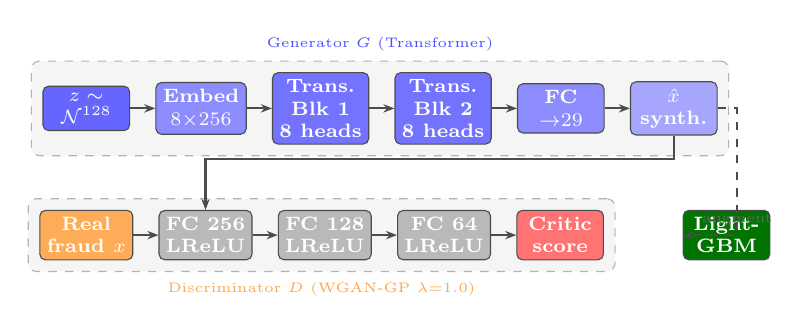
\begin{tikzpicture}[node distance=0.38cm and 0.32cm]
  %% Generator row
  \node[block=blue!60] (z)    {$z \sim$\\$\mathcal{N}^{128}$};
  \node[block=blue!45, right=of z]   (emb)  {Embed\\$8{\times}256$};
  \node[block=blue!55, right=of emb] (tf1)  {Trans.\\Blk 1\\8 heads};
  \node[block=blue!55, right=of tf1] (tf2)  {Trans.\\Blk 2\\8 heads};
  \node[block=blue!45, right=of tf2] (proj) {FC\\${\to}29$};
  \node[block=blue!35, right=of proj](synx) {$\hat{x}$\\synth.};
  \foreach \a/\b in {z/emb,emb/tf1,tf1/tf2,tf2/proj,proj/synx}
    \draw[arr] (\a) -- (\b);
  \begin{scope}[on background layer]
    \node[grpbox, fit=(z)(emb)(tf1)(tf2)(proj)(synx),
      label={[font=\tiny,text=blue!70]above:Generator $G$ (Transformer)}] {};
  \end{scope}
  %% Discriminator row
  \node[block=orange!65, below=1.0cm of z]  (xr)  {Real\\fraud $x$};
  \node[block=gray!55, right=of xr]         (d256){FC 256\\LReLU};
  \node[block=gray!55, right=of d256]       (d128){FC 128\\LReLU};
  \node[block=gray!55, right=of d128]       (d64) {FC 64\\LReLU};
  \node[block=red!55,  right=of d64]        (dout){Critic\\score};
  \foreach \a/\b in {xr/d256,d256/d128,d128/d64,d64/dout}
    \draw[arr] (\a) -- (\b);
  \draw[arr] (synx.south) -- ++(0,-0.3) -| (d256.north);
  \begin{scope}[on background layer]
    \node[grpbox, fit=(xr)(d256)(d128)(d64)(dout),
      label={[font=\tiny,text=orange!70]below:Discriminator $D$ (WGAN-GP $\lambda{=}1.0$)}] {};
  \end{scope}
  %% LightGBM
  \node[block=green!45!black, right=1.0cm of dout](lgb){Light-\\GBM};
  \draw[arr, dashed] (synx.east) -- ++(0.25,0) |- (lgb.west)
    node[midway,lbl,above]{augment};
\end{tikzpicture}}
\caption{T-GAN. Transformer encoder captures long-range feature interactions
across the 29-dimensional fraud feature space. Synthetic samples augment
the LightGBM training set.}
\label{fig:tgan}
\end{figure}

\subsubsection{R-GAN (Regularized GAN)}

The R-GAN generator maps a 128-dimensional latent vector through three
fully connected layers (256-512-256) with spectral normalization on all
linear weights, BatchNorm1d, and CELU activations, projecting to 29 output
features (V1--V28 + Amount) with no final activation. Spectral normalization
constrains the Lipschitz constant of each layer, providing an additional
stability mechanism on top of the WGAN-GP gradient penalty. The discriminator
(critic) is a three-layer network (512-256-128) with spectral normalization
and LeakyReLU(0.2), no BatchNorm, returning both a scalar critic score and
intermediate feature representations. The distinguishing component is the
Similarity Measure Loss, which regularizes the generator with two terms:
(1) a statistical penalty on the per-feature mean and standard deviation
difference between synthetic and real fraud batches, and (2) a feature
matching penalty on discriminator intermediate representations:
\begin{equation}
\mathcal{L}_\text{sim} = \text{MSE}(\mu_\text{syn}, \mu_\text{real})
  + \text{MSE}(\sigma_\text{syn}, \sigma_\text{real})
  + \text{MSE}(f_D(\hat{x}), f_D(x))
\end{equation}
where $f_D(\cdot)$ denotes discriminator intermediate features and
$\lambda_\text{sim}=0.5$ weights this term in the total generator loss.
Training uses WGAN-GP ($\lambda=10.0$, 5 critic steps) with Adam
($\text{lr}=10^{-4}$, $\beta=(0.5, 0.9)$) for 300 epochs with early
stopping (patience 25).

\begin{figure}[htbp]
\centering
\resizebox{\columnwidth}{!}{%
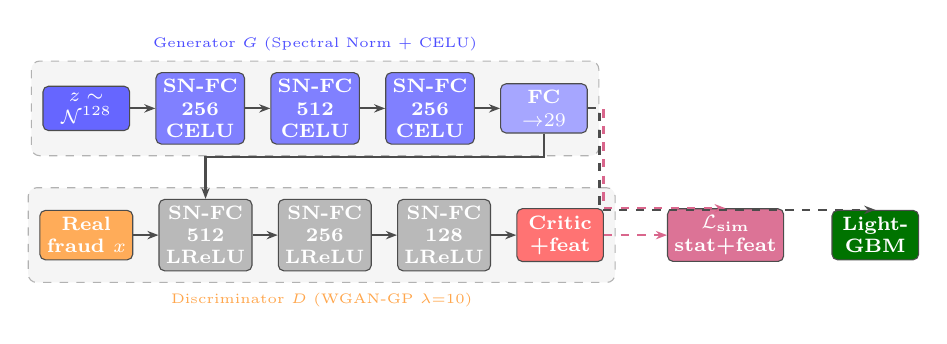
\begin{tikzpicture}[node distance=0.38cm and 0.32cm]
  %% Generator row
  \node[block=blue!60] (z)    {$z \sim$\\$\mathcal{N}^{128}$};
  \node[block=blue!50, right=of z]   (g1) {SN-FC\\256\\CELU};
  \node[block=blue!50, right=of g1]  (g2) {SN-FC\\512\\CELU};
  \node[block=blue!50, right=of g2]  (g3) {SN-FC\\256\\CELU};
  \node[block=blue!35, right=of g3]  (gout){FC\\${\to}29$};
  \foreach \a/\b in {z/g1,g1/g2,g2/g3,g3/gout}
    \draw[arr] (\a) -- (\b);
  \begin{scope}[on background layer]
    \node[grpbox, fit=(z)(g1)(g2)(g3)(gout),
      label={[font=\tiny,text=blue!70]above:Generator $G$ (Spectral Norm + CELU)}] {};
  \end{scope}
  %% Discriminator row
  \node[block=orange!65, below=1.0cm of z] (xr)  {Real\\fraud $x$};
  \node[block=gray!55, right=of xr]        (d512){SN-FC\\512\\LReLU};
  \node[block=gray!55, right=of d512]      (d256){SN-FC\\256\\LReLU};
  \node[block=gray!55, right=of d256]      (d128){SN-FC\\128\\LReLU};
  \node[block=red!55,  right=of d128]      (dout){Critic\\+feat};
  \foreach \a/\b in {xr/d512,d512/d256,d256/d128,d128/dout}
    \draw[arr] (\a) -- (\b);
  \draw[arr] (gout.south) -- ++(0,-0.3) -| (d512.north);
  \begin{scope}[on background layer]
    \node[grpbox, fit=(xr)(d512)(d256)(d128)(dout),
      label={[font=\tiny,text=orange!70]below:Discriminator $D$ (WGAN-GP $\lambda{=}10$)}] {};
  \end{scope}
  %% Sim Loss
  \node[block=purple!55, right=0.8cm of dout](sim){$\mathcal{L}_\text{sim}$\\stat+feat};
  \draw[arr, dashed, purple!60] (dout.east) -- (sim.west);
  \draw[arr, dashed, purple!60] (gout.east) -- ++(0.2,0) |- (sim.north);
  %% LightGBM
  \node[block=green!45!black, right=0.6cm of sim](lgb){Light-\\GBM};
  \draw[arr, dashed] (gout.east) -- ++(0.15,0) |- (lgb.north);
\end{tikzpicture}}
\caption{R-GAN. Spectral normalization on all linear layers and CELU activations
stabilize training. The Similarity Measure Loss constrains synthetic samples
to match the statistical distribution and discriminator feature space of real
fraud.}
\label{fig:rgan}
\end{figure}

\subsubsection{CTGAN}

CTGAN addresses non-Gaussian, multi-modal continuous variables in tabular
data. Unlike the other Pipeline A models, CTGAN trains on all 51 engineered
features natively, as its Variational Gaussian Mixture (VGM) transformer
handles distributional normalization column-wise before any network training.
Each continuous feature is decomposed into a mixture of Gaussians; the
generator is conditioned on mode membership per column, enabling accurate
synthesis of skewed and heavy-tailed distributions. The generator and
discriminator are each two-layer feedforward networks with hidden dimensions
$(256, 256)$ and embedding dimension 128. The discriminator uses PacGAN with
packing factor $k=10$, concatenating 10 samples per discriminator forward
pass to prevent mode collapse on tabular data. A conditional vector encoding
\texttt{Class}~=~1 ensures every generated sample belongs to the fraud class.
Training runs for 300 epochs, batch size 500, Adam with
$\text{lr}=2\times10^{-4}$ and $\beta=(0.5, 0.9)$.

\begin{figure}[htbp]
\centering
\resizebox{\columnwidth}{!}{%
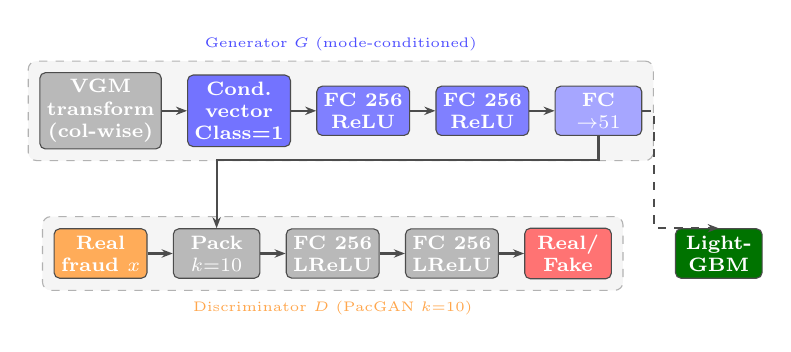
\begin{tikzpicture}[node distance=0.38cm and 0.32cm]
  %% VGM preprocessing
  \node[block=gray!55] (vgm) {VGM\\transform\\(col-wise)};
  \node[block=blue!55, right=of vgm] (cond){Cond.\\vector\\Class=1};
  %% Generator
  \node[block=blue!50, right=of cond]  (g1) {FC 256\\ReLU};
  \node[block=blue!50, right=of g1]    (g2) {FC 256\\ReLU};
  \node[block=blue!35, right=of g2]    (gout){FC\\${\to}51$};
  \draw[arr] (vgm) -- (cond);
  \foreach \a/\b in {cond/g1,g1/g2,g2/gout}
    \draw[arr] (\a) -- (\b);
  \begin{scope}[on background layer]
    \node[grpbox, fit=(vgm)(cond)(g1)(g2)(gout),
      label={[font=\tiny,text=blue!70]above:Generator $G$ (mode-conditioned)}] {};
  \end{scope}
  %% Discriminator
  \node[block=orange!65, below=1.0cm of vgm] (xr)  {Real\\fraud $x$};
  \node[block=gray!55, right=of xr]          (pac) {Pack\\$k{=}10$};
  \node[block=gray!55, right=of pac]         (d256a){FC 256\\LReLU};
  \node[block=gray!55, right=of d256a]       (d256b){FC 256\\LReLU};
  \node[block=red!55,  right=of d256b]       (dout){Real/\\Fake};
  \foreach \a/\b in {xr/pac,pac/d256a,d256a/d256b,d256b/dout}
    \draw[arr] (\a) -- (\b);
  \draw[arr] (gout.south) -- ++(0,-0.3) -| (pac.north);
  \begin{scope}[on background layer]
    \node[grpbox, fit=(xr)(pac)(d256a)(d256b)(dout),
      label={[font=\tiny,text=orange!70]below:Discriminator $D$ (PacGAN $k{=}10$)}] {};
  \end{scope}
  %% LightGBM
  \node[block=green!45!black, right=0.8cm of dout](lgb){Light-\\GBM};
  \draw[arr, dashed] (gout.east) -- ++(0.15,0) |- (lgb.north);
\end{tikzpicture}}
\caption{CTGAN. Column-wise VGM transforms handle non-Gaussian feature
distributions. PacGAN packing ($k=10$) prevents mode collapse. All 51
engineered features are synthesized natively.}
\label{fig:ctgan}
\end{figure}

\subsubsection{GANomaly}

GANomaly implements an encoder-decoder-encoder architecture for
semi-supervised anomaly detection, trained exclusively on normal transactions.
The first encoder $E_1$ maps the 50-dimensional input to a 32-dimensional
latent vector $z$ through two fully connected layers (256, 128) with
BatchNorm1d and LeakyReLU(0.2). The decoder $G$ reconstructs the input
$\hat{x}$ from $z$ through a mirrored structure (128, 256) with BatchNorm
and ReLU, no final activation. The second encoder $E_2$ re-encodes $\hat{x}$
to produce $\hat{z}$. The anomaly score is $\|z - \hat{z}\|_2$: normal
transactions are reconstructed faithfully ($z \approx \hat{z}$) while fraud
deviates from the learned normal manifold. The discriminator is a two-layer
network (128-64) with LeakyReLU returning a real/fake logit and intermediate
features. The generator loss combines:
\begin{equation}
\mathcal{L}_G = w_\text{adv}\,\mathcal{L}_\text{adv}
              + w_\text{con}\,\|x - \hat{x}\|_1
              + w_\text{enc}\,\|z - \hat{z}\|_2^2
\end{equation}
with $w_\text{adv}=1.0$, $w_\text{con}=50.0$, $w_\text{enc}=1.0$. Training
uses Adam ($\text{lr}=10^{-4}$, $\beta=(0.5, 0.999)$), batch 256, 100 epochs.
The anomaly threshold is set at the 95th percentile of validation normal
scores.

\begin{figure}[htbp]
\centering
\resizebox{\columnwidth}{!}{%
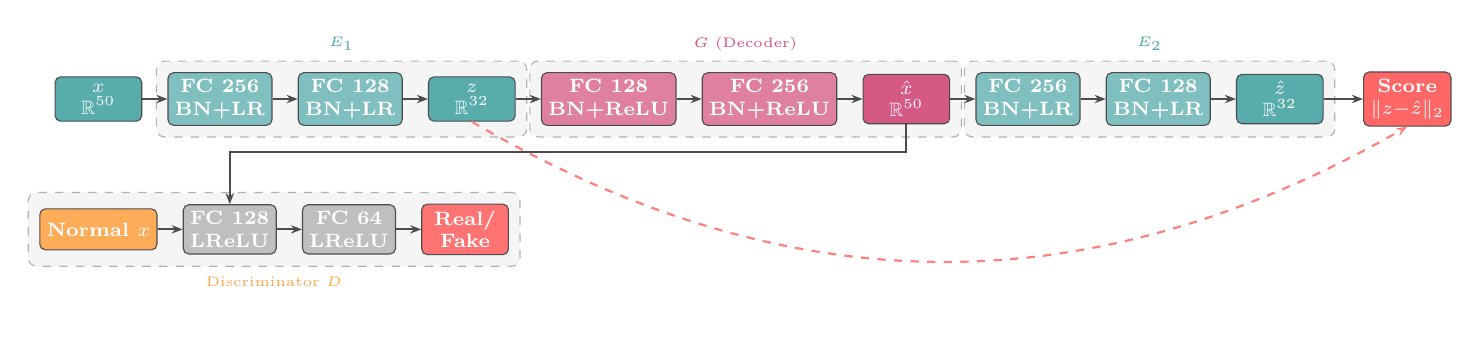
\begin{tikzpicture}[node distance=0.38cm and 0.32cm]
  %% Top row: E1 -> G -> E2
  \node[block=teal!65]  (x)    {$x$\\$\mathbb{R}^{50}$};
  \node[block=teal!50, right=of x]   (e1a)  {FC 256\\BN+LR};
  \node[block=teal!50, right=of e1a] (e1b)  {FC 128\\BN+LR};
  \node[block=teal!65, right=of e1b] (z)    {$z$\\$\mathbb{R}^{32}$};
  \node[block=purple!50, right=of z]  (da)  {FC 128\\BN+ReLU};
  \node[block=purple!50, right=of da] (db)  {FC 256\\BN+ReLU};
  \node[block=purple!65, right=of db] (xh)  {$\hat{x}$\\$\mathbb{R}^{50}$};
  \node[block=teal!50, right=of xh]  (e2a)  {FC 256\\BN+LR};
  \node[block=teal!50, right=of e2a] (e2b)  {FC 128\\BN+LR};
  \node[block=teal!65, right=of e2b] (zh)   {$\hat{z}$\\$\mathbb{R}^{32}$};
  \foreach \a/\b in {x/e1a,e1a/e1b,e1b/z,z/da,da/db,db/xh,xh/e2a,e2a/e2b,e2b/zh}
    \draw[arr] (\a) -- (\b);
  \begin{scope}[on background layer]
    \node[grpbox, fit=(e1a)(e1b)(z), label={[font=\tiny,text=teal!70]above:$E_1$}] {};
    \node[grpbox, fit=(da)(db)(xh),  label={[font=\tiny,text=purple!70]above:$G$ (Decoder)}] {};
    \node[grpbox, fit=(e2a)(e2b)(zh),label={[font=\tiny,text=teal!70]above:$E_2$}] {};
  \end{scope}
  %% Anomaly score
  \node[block=red!60, right=0.5cm of zh] (score){Score\\$\|z{-}\hat{z}\|_2$};
  \draw[arr] (zh.east) -- (score.west);
  \draw[arr, dashed, red!50, bend right=30] (z.south) to (score.south);
  %% Discriminator row
  \node[block=orange!65, below=1.1cm of x]  (xnorm){Normal $x$};
  \node[block=gray!50,   right=of xnorm]    (dc1)  {FC 128\\LReLU};
  \node[block=gray!50,   right=of dc1]      (dc2)  {FC 64\\LReLU};
  \node[block=red!55,    right=of dc2]      (dout) {Real/\\Fake};
  \foreach \a/\b in {xnorm/dc1,dc1/dc2,dc2/dout}
    \draw[arr] (\a) -- (\b);
  \draw[arr] (xh.south) -- ++(0,-0.35) -| (dc1.north);
  \begin{scope}[on background layer]
    \node[grpbox, fit=(xnorm)(dc1)(dc2)(dout),
      label={[font=\tiny,text=orange!70]below:Discriminator $D$}] {};
  \end{scope}
\end{tikzpicture}}
\caption{GANomaly. The dual-encoder structure ($E_1$, $E_2$) measures latent
space consistency: the anomaly score $\|z-\hat{z}\|_2$ is low for normal
transactions and elevated when fraud cannot be faithfully reconstructed.}
\label{fig:ganomaly}
\end{figure}

\subsubsection{Skip-GANomaly}

Skip-GANomaly augments the GANomaly encoder-decoder with U-Net skip
connections. The encoder maps the 50-dimensional input through four layers
(256-128-64-32) with BatchNorm1d and LeakyReLU(0.2), storing the output of
each intermediate layer as a skip connection. The decoder mirrors this
structure (64-128-256-50) with ReLU, concatenating the corresponding encoder
skip outputs to each decoder input. This doubles the decoder's effective
input width at each layer, preserving fine-grained local feature patterns
that are otherwise discarded during compression. The discriminator is a
two-layer network (128-64) with LeakyReLU, returning a real/fake logit and
intermediate features for feature-matching loss. The anomaly score is:
\begin{equation}
s(x) = 0.9\,\mathcal{L}_\text{rec}(x, \hat{x}) + 0.1\,\mathcal{L}_\text{feat}(x, \hat{x})
\end{equation}
where $\mathcal{L}_\text{rec} = \|x - \hat{x}\|_2^2$ and
$\mathcal{L}_\text{feat} = \|f_D(x) - f_D(\hat{x})\|_2^2$. Training loss
weights are $w_\text{rec}=1.0$, $w_\text{feat}=1.0$, $w_\text{adv}=0.001$,
with Adam ($\text{lr}=10^{-4}$, $\beta=(0.5, 0.999)$), 100 epochs.

\begin{figure}[htbp]
\centering
\resizebox{\columnwidth}{!}{%
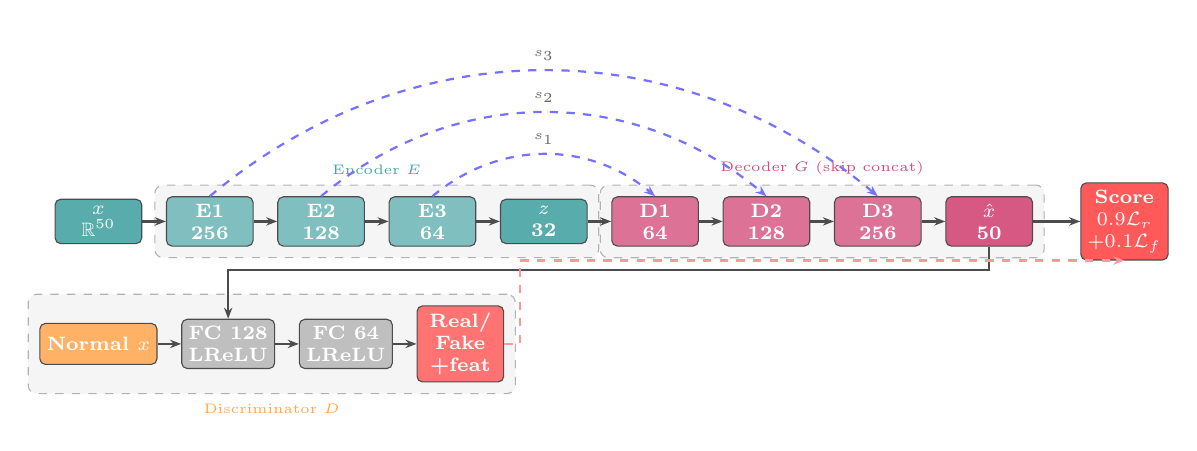
\begin{tikzpicture}[node distance=0.36cm and 0.30cm]
  %% Input
  \node[block=teal!65] (x) {$x$\\$\mathbb{R}^{50}$};
  %% Encoder
  \node[block=teal!50, right=of x]  (e1) {E1\\256};
  \node[block=teal!50, right=of e1] (e2) {E2\\128};
  \node[block=teal!50, right=of e2] (e3) {E3\\64};
  \node[block=teal!65, right=of e3] (z)  {$z$\\32};
  \foreach \a/\b in {x/e1,e1/e2,e2/e3,e3/z}
    \draw[arr] (\a) -- (\b);
  \begin{scope}[on background layer]
    \node[grpbox, fit=(e1)(e2)(e3)(z),
      label={[font=\tiny,text=teal!70]above:Encoder $E$}] {};
  \end{scope}
  %% Decoder
  \node[block=purple!55, right=of z]  (d1) {D1\\64};
  \node[block=purple!55, right=of d1] (d2) {D2\\128};
  \node[block=purple!55, right=of d2] (d3) {D3\\256};
  \node[block=purple!65, right=of d3] (xh) {$\hat{x}$\\50};
  \foreach \a/\b in {z/d1,d1/d2,d2/d3,d3/xh}
    \draw[arr] (\a) -- (\b);
  \begin{scope}[on background layer]
    \node[grpbox, fit=(d1)(d2)(d3)(xh),
      label={[font=\tiny,text=purple!70]above:Decoder $G$ (skip concat)}] {};
  \end{scope}
  %% Skip connections
  \draw[arr, dashed, blue!55, bend left=40]
    (e3.north) to node[lbl,above]{$s_1$} (d1.north);
  \draw[arr, dashed, blue!55, bend left=40]
    (e2.north) to node[lbl,above]{$s_2$} (d2.north);
  \draw[arr, dashed, blue!55, bend left=40]
    (e1.north) to node[lbl,above]{$s_3$} (d3.north);
  %% Anomaly score
  \node[block=red!65, right=0.6cm of xh] (score)
    {Score\\$0.9\mathcal{L}_r$\\$+0.1\mathcal{L}_f$};
  \draw[arr] (xh.east) -- (score.west);
  %% Discriminator row
  \node[block=orange!60, below=1.0cm of x]  (xr)   {Normal $x$};
  \node[block=gray!50,   right=of xr]       (dc1)  {FC 128\\LReLU};
  \node[block=gray!50,   right=of dc1]      (dc2)  {FC 64\\LReLU};
  \node[block=red!55,    right=of dc2]      (dout) {Real/\\Fake\\+feat};
  \foreach \a/\b in {xr/dc1,dc1/dc2,dc2/dout}
    \draw[arr] (\a) -- (\b);
  \draw[arr] (xh.south) -- ++(0,-0.3) -| (dc1.north);
  \draw[arr, dashed, red!40] (dout.east) -- ++(0.2,0) |- (score.south);
  \begin{scope}[on background layer]
    \node[grpbox, fit=(xr)(dc1)(dc2)(dout),
      label={[font=\tiny,text=orange!70]below:Discriminator $D$}] {};
  \end{scope}
\end{tikzpicture}}
\caption{Skip-GANomaly. Three U-Net skip connections ($s_1, s_2, s_3$)
concatenate encoder outputs to decoder inputs, preserving local feature
structure. The weighted anomaly score combines reconstruction and
feature-matching error.}
\label{fig:sgan}
\end{figure}

\subsubsection{f-AnoGAN}

f-AnoGAN proceeds in two independent training phases. \textbf{Phase~1
(WGAN-GP)} trains a generator $G$ mapping a 64-dimensional latent vector
$z \sim \mathcal{N}(0,I)$ to 50 output features through two fully connected
layers (256-512) with BatchNorm1d and ReLU, no final activation. The
discriminator (critic) uses two layers (512-256) with LeakyReLU(0.2), no
BatchNorm, returning a critic score and intermediate features. WGAN-GP is
used with $\lambda=10$, 5 critic steps per generator update, Adam
($\text{lr}=10^{-4}$, $\beta=(0.5, 0.9)$), 100 epochs. \textbf{Phase~2
(Encoder training)} freezes $G$ and $D$, then trains a separate encoder $E$
- two layers (256-512) with BatchNorm1d and LeakyReLU - to invert the
generator:
\begin{equation}
\mathcal{L}_E = \|x - G(E(x))\|_2^2 + \kappa\,\|f_D(x) - f_D(G(E(x)))\|_2^2
\end{equation}
with $\kappa=1.0$, early stopping (patience 10) on encoder loss over 50
epochs. At inference, the anomaly score is computed in a single forward pass,
eliminating the per-sample iterative optimization of vanilla AnoGAN:
\begin{equation}
s(x) = \|x - G(E(x))\|_2 + \kappa\,\|f_D(x) - f_D(G(E(x)))\|_2
\end{equation}
Scores are Z-score normalized using validation normal statistics; the
threshold is set at the 95th percentile of validation normal scores,
giving a 5\% false-positive rate on normal transactions by construction.

\begin{figure}[htbp]
\centering
\resizebox{\columnwidth}{!}{%
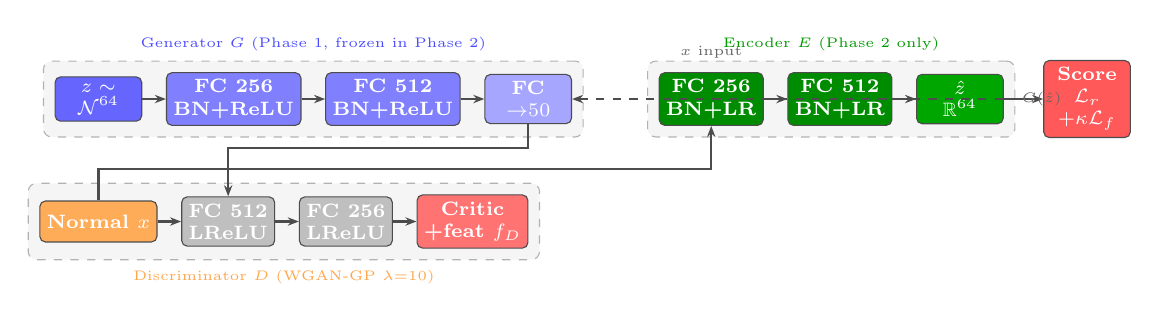
\begin{tikzpicture}[node distance=0.36cm and 0.30cm]
  %% Phase 1: WGAN-GP
  \node[block=blue!60] (z)    {$z \sim$\\$\mathcal{N}^{64}$};
  \node[block=blue!50, right=of z]   (g1)  {FC 256\\BN+ReLU};
  \node[block=blue!50, right=of g1]  (g2)  {FC 512\\BN+ReLU};
  \node[block=blue!35, right=of g2]  (gout){FC\\${\to}50$};
  \foreach \a/\b in {z/g1,g1/g2,g2/gout}
    \draw[arr] (\a) -- (\b);
  \begin{scope}[on background layer]
    \node[grpbox, fit=(z)(g1)(g2)(gout),
      label={[font=\tiny,text=blue!70]above:Generator $G$ (Phase 1, frozen in Phase 2)}] {};
  \end{scope}
  %% Discriminator
  \node[block=orange!65, below=1.0cm of z] (xr)  {Normal $x$};
  \node[block=gray!50, right=of xr]        (dc1) {FC 512\\LReLU};
  \node[block=gray!50, right=of dc1]       (dc2) {FC 256\\LReLU};
  \node[block=red!55,  right=of dc2]       (dout){Critic\\+feat $f_D$};
  \foreach \a/\b in {xr/dc1,dc1/dc2,dc2/dout}
    \draw[arr] (\a) -- (\b);
  \draw[arr] (gout.south) -- ++(0,-0.3) -| (dc1.north);
  \begin{scope}[on background layer]
    \node[grpbox, fit=(xr)(dc1)(dc2)(dout),
      label={[font=\tiny,text=orange!70]below:Discriminator $D$ (WGAN-GP $\lambda{=}10$)}] {};
  \end{scope}
  %% Phase 2: Encoder
  \node[block=green!55!black, right=1.1cm of gout] (e1) {FC 256\\BN+LR};
  \node[block=green!55!black, right=of e1]          (e2) {FC 512\\BN+LR};
  \node[block=green!65!black, right=of e2]          (zh) {$\hat{z}$\\$\mathbb{R}^{64}$};
  \foreach \a/\b in {e1/e2,e2/zh}
    \draw[arr] (\a) -- (\b);
  \node[lbl, above=0.05cm of e1] (enc_input) {$x$ input};
  \draw[arr] (xr.north) -- ++(0,0.4) -| (e1.south);
  \begin{scope}[on background layer]
    \node[grpbox, fit=(e1)(e2)(zh),
      label={[font=\tiny,text=green!60!black]above:Encoder $E$ (Phase 2 only)}] {};
  \end{scope}
  %% Inference score
  \node[block=red!65, right=0.5cm of zh] (score){Score\\$\mathcal{L}_r$\\$+\kappa\mathcal{L}_f$};
  \draw[arr] (zh.east) -- (score.west);
  \draw[arr, dashed] (zh.east) -- ++(0.1,0) |- (gout.east)
    node[near start, lbl, right]{$G(\hat{z})$};
\end{tikzpicture}}
\caption{f-AnoGAN. Phase~1 trains the WGAN-GP; Phase~2 trains the encoder
$E$ with $G$ and $D$ frozen. At inference, a single forward pass through
$E \to G$ replaces the iterative optimization of vanilla AnoGAN.}
\label{fig:fanogan}
\end{figure}

\subsection{Evaluation Protocol}

All models are evaluated against the same 492-record fraud holdout set,
never exposed to any model during training. Metrics reported are F1-score,
Precision, Recall, AUROC, and inference latency. Statistical significance
of cross-paradigm performance differences will be assessed using the
Wilcoxon Signed-Rank Test across 5-fold cross-validation results, testing
the null hypothesis $H_0$ that median F1-scores are equal between paradigms.

\subsection{Reproducibility}

All randomness sources are seeded from a single global seed (42) via
deterministic SHA-256-derived component seeds. The experiment fingerprint
\texttt{c04ea4ba} uniquely identifies this configuration. All code runs
on Kaggle Notebooks (CPU); experiment tracking via Weights \& Biases
(W\&B project: \textit{PRINCIPLES AND ENGINEERING APPLICATIONS OF AI}).

%--------
\section{Results}

\subsection{Holdout Evaluation}

Table~\ref{tab:results} presents results for all six models evaluated on
the same 492-record fraud holdout combined with 5,000 normal validation
samples.

\begin{table}[htbp]
\caption{Holdout Evaluation Results (492 Fraud + 5,000 Normal)}
\label{tab:results}
\centering
\begin{tabular}{lccccr}
\toprule
\textbf{Model} & \textbf{F1} & \textbf{Prec.} & \textbf{Rec.}
               & \textbf{AUROC} & \textbf{Lat.\ (ms)} \\
\midrule
\multicolumn{6}{l}{\textit{Pipeline A — Generative Augmentation}} \\
T-GAN + LGB   & 0.9328 & 1.0000 & 0.8740 & 0.9998 & 11.1 \\
CTGAN + LGB   & 0.9199 & 1.0000 & 0.8516 & 0.9999 & 10.9 \\
R-GAN + LGB   & 0.9954 & 0.9983 & 0.9926 & 0.9999 &  9.8 \\
\midrule
\multicolumn{6}{l}{\textit{Pipeline B — Reconstruction Detection}} \\
Skip-GANomaly & 0.8742 & 0.9372 & 0.8191 & 0.9821 & 25.8 \\
GANomaly      & 0.8025 & 0.7186 & 0.9085 & 0.9892 & 14.6 \\
f-AnoGAN      & 0.7649 & 0.6453 & 0.9390 & 0.9907 & 14.9 \\
\bottomrule
\end{tabular}
\end{table}

\subsection{Training Dynamics}

\textbf{T-GAN} exhibited stable WGAN-GP convergence over 260 epochs. Gradient
penalty loss decreased from 1.59 to 0.79, indicating convergence without mode
collapse. Synthetic quality gates: MMD~=~0.0042 (PASS); JSD~=~0.2035 (FAIL);
novelty~=~18,152 (PASS); discriminator AUC~=~0.9946 (FAIL). Despite JSD and
discriminator AUC failures, the downstream classifier achieves F1~=~0.9328
and AUROC~=~0.9998.

\textbf{R-GAN} converged stably over 300 epochs with the Similarity Measure
Loss providing additional regularization on top of the WGAN-GP objective.
Spectral normalization on all linear layers prevented gradient explosion
without requiring gradient clipping. Synthetic quality gate results show the
same JSD and discriminator AUC failures as T-GAN; the Similarity Loss
improves statistical fidelity (lower JSD than T-GAN) but does not bring
either model within the quality gate thresholds. The downstream classifier
achieves the strongest Pipeline A performance: F1~=~0.9954, Precision~=~0.9983,
Recall~=~0.9926.

\textbf{CTGAN} trained for 300 epochs; generator loss decreased from $+4.2$
to $+1.8$, discriminator loss remained bounded near $-1.0$. Synthetic quality
gates: MMD~=~0.0042 (PASS); JSD~=~0.2641 (FAIL); novelty~=~60,599 (PASS);
discriminator AUC~=~0.9996 (FAIL). CTGAN produces substantially more novel
samples (novelty distance 60,599 vs.\ 18,152 for T-GAN), consistent with its
mode-conditioned synthesis of the full 51-feature space. Despite identical
gate failures, AUROC~=~0.9999 is the highest across all six models.

\textbf{Skip-GANomaly} converged over 100 epochs; discriminator loss
decreased from 0.6925 to 0.5670, approaching the theoretical optimum of 0.5.
Reconstruction loss stabilized at 0.0039 by epoch 40.

\textbf{GANomaly} converged over 100 epochs; context loss
$\mathcal{L}_\text{con}$ (weight 50) dominated and decreased consistently.
Encoder consistency loss $\mathcal{L}_\text{enc}$ decreased toward zero,
confirming $E_2(\hat{x}) \approx E_1(x)$ for normal inputs. Inference
latency of 14.6~ms is $1.8\times$ faster than Skip-GANomaly (25.8~ms),
attributable to the absence of skip-connection feature aggregation.

\textbf{f-AnoGAN} Phase~1 WGAN-GP converged over 100 epochs; gradient
penalty stabilized near 1.0 by epoch 30. Phase~2 encoder training converged
within 50 epochs with both $\mathcal{L}_\text{rec}$ and
$\mathcal{L}_\text{feat}$ decreasing monotonically. Anomaly score inversion
check returned raw AUROC~$>0.5$, confirming correct score orientation.
f-AnoGAN achieves the highest recall of all Pipeline~B models (0.9390) and
the highest AUROC within Pipeline~B (0.9907), at the cost of lower precision
(0.6453) from the 95th-percentile liberal threshold strategy.

\subsection{Cross-Paradigm Comparison}

Pipeline~A dominates Pipeline~B on F1 and Precision across all model pairs.
The best Pipeline~A model (R-GAN, F1~=~0.9954) exceeds the best Pipeline~B
model (Skip-GANomaly, F1~=~0.8742) by 0.1212 F1 points. Within Pipeline~B,
f-AnoGAN achieves the highest recall (0.9390) and AUROC (0.9907), confirming
that reconstruction-based models with liberal thresholds achieve near-complete
fraud capture at the cost of precision. Pipeline~A inference latency
($\sim$10~ms) is $1.8$--$2.6\times$ faster than Pipeline~B ($14.6$--$25.8$~ms)
due to the LightGBM classifier's efficient tree evaluation versus neural
reconstruction forward passes.

%--------
\section{Discussion and Analysis}

\subsection{Effect of Feature Scaling on GAN Training}

All six models required explicit StandardScaler preprocessing with $\pm5\sigma$
clipping, despite the upstream RobustScaler applied in Stage~2. The Stage~2
scaler normalizes only \texttt{Amount}; the 20 engineered features added in
Stage~3 (rolling velocity counts, amount z-scores, cyclical time signals)
introduce high-magnitude values not covered by the original scaler.
Unscaled inputs caused loss explosion in all neural network models. CTGAN
is the exception: its VGM transformer performs column-wise normalization
internally, but the pattern of needing a separate scaling pass before all
PyTorch-based models is consistent across both pipelines.

\subsection{Quality Gates vs. Classifier Performance}

All three Pipeline~A GANs fail JSD and discriminator AUC quality gates yet
achieve AUROC $\geq 0.9998$. This pattern holds across architecturally
distinct generators (Transformer, spectral-norm feedforward, VGM-conditioned
CTGAN), suggesting the failure is structural rather than model-specific. The
quality gate metrics measure distributional realism in the raw feature space;
classifier performance depends on decision boundary separability in a
high-dimensional learned representation. A synthetic sample that is
statistically distinguishable from real fraud in the original 29-dimensional
GAN feature space may still provide informative signal in the 51-dimensional
feature space where LightGBM operates. This decoupling of synthetic fidelity
from downstream utility is a consistent finding across all three Pipeline~A
models.

\subsection{Precision-Recall Trade-off Between Paradigms}

Pipeline~A achieves perfect or near-perfect precision (1.0000, 1.0000,
0.9983) with lower recall (0.8516--0.9926), while Pipeline~B achieves
higher recall (0.8191--0.9390) at lower precision (0.6453--0.9372). This
reflects the fundamental difference in how each paradigm sets its decision
boundary. LightGBM classifiers output calibrated probabilities enabling
high-confidence threshold selection; reconstruction-based anomaly scores
are unnormalized and threshold selection via validation-normal percentiles
inherits sensitivity to the score distribution shift when fraud is introduced
in the evaluation set. GANomaly and f-AnoGAN both use a 95th-percentile
threshold strategy that accepts false positives to maximize recall - an
operationally sensible choice for fraud detection but architecturally
constrained by the lack of label-aware training.

\subsection{Inference Latency Trade-off}

Pipeline~A inference cost ($9.8$--$11.1$~ms for 5,492 records) reflects
LightGBM's tree evaluation. Pipeline~B cost ($14.6$--$25.8$~ms) reflects
neural reconstruction forward passes. Skip-GANomaly's $25.8$~ms is the
slowest, attributable to skip-connection feature aggregation at each decoder
layer. f-AnoGAN's single-pass encoder design achieves near-parity with
GANomaly ($14.9$ vs.\ $14.6$~ms), confirming that the encoder successfully
eliminates the iterative optimization overhead of vanilla AnoGAN.

\section*{Code and Experiment Tracking}

All source code is publicly available at:
\begin{center}
\href{https://github.com/kkipngenokoech/synthesize-or-reconstruct}{\texttt{github repo}}
\end{center}

\noindent Experiment runs, training curves, and per-epoch metrics are logged via
Weights \& Biases. Two W\&B projects were used during development:
\begin{itemize}
  \item Pipeline A (T-GAN, LightGBM):\;
        \href{https://wandb.ai/kkipngenokoech-carnegie-mellon-university/PRINCIPLES%20AND%20ENGINEERING%20APPLICATIONS%20OF%20AI?nw=nwuserkkipngenokoech}{\texttt{W\&B: Pipeline A}}
  \item Pipeline B (Skip-GANomaly):\;
        \href{https://wandb.ai/kkipngenokoech-carnegie-mellon-university/PRINCIPLES%20AND%20ENGINEERING%20%20APPLICATIONS%20OF%20AI?nw=nwuserkkipngenokoech}{\texttt{W\&B: Pipeline B}}
\end{itemize}

%--------
\section{Conclusion and Future Work}

Pipeline~A (generative
augmentation) outperforms Pipeline~B (reconstruction-based detection)
on F1 and Precision across all model pairs, with R-GAN + LightGBM
achieving the strongest single-model result (F1~=~0.9954, AUROC~=~0.9999).
Pipeline~B models achieve higher recall at lower precision, reflecting
the structural consequence of unsupervised threshold selection and
label-free training.

\noindent Remaining work comprises:
\begin{itemize}
    \item[-] executing the Wilcoxon Signed-Rank Test
across all six models to formally assess statistical significance of
the cross-paradigm F1 gap
\item[-] Investigating whether quality gate
failures (JSD, discriminator AUC) across all three Pipeline~A models
can be resolved through extended training without degrading classifier
performance
\item[-] Expand our validation across other imbalanced financial datasets to assess generalizability 
\item[-] Evaluating adversarial robustness - the degree
to which each paradigm is susceptible to adversarial examples designed
to evade detection.
\item[-] How the best model can contribute in fraud detection as an improvement of the commercial already existing fraud detectors.
\end{itemize}
\noident The consistent finding that synthetic quality gate compliance does not
predict downstream classifier utility across three architecturally
distinct generators warrants formal investigation in the final report.

%--------
\bibliographystyle{IEEEtran}
\bibliography{references}

\end{document}